\chapter{Introduction}
\section{Parallel sparse matrix-vector multiplication}
Matrices are one of the most important mathematical objects, as they can be used to represent a wide variety of data in many scientific disciplines: they can encode the structure of a graph, define Markov chains with finitely many states, or maybe represent linear combinations of quantum states or also the behaviour of electronic components. 

In most real-world computations, the systems considered are usually of very large size and involve \textbf{sparse} matrices, because the analyzed variables are usually connected to a limited number of others (for example, a very large graph in which each node has just a handful of incident edges); therefore, the matrices involved have the vast majority of entries equal to 0.

More formally, let us consider a matrix of size $m \times n$ with $N$ nonzeros. We say that the matrix is sparse if $ N \ll mn $.

One of the most fundamental operations performed in these real-world computations is the sparse matrix-vector multiplication: in which we compute

\begin{align}
	u:=Av
	\label{uAv}
\end{align}
where $A$ denotes our $m \times n$ sparse matrix, $v$ denotes a $n \times 1$ dense vector, and $u$ the resulting $m \times 1$ vector.

Computing this quantity following the definition of matrix-vector multiplication, i.e. with the sum 

\[ 
	u_i = \sum_{j=0}^{n-1} a_{ij} v_j \qquad 0 \leq i < m 
\]

requires $\mathcal{O}(n^2) = \mathcal{O}(mn)$ operations; this is not very efficient if we have a sparse matrix: if we perform the multiplications only on the nonzero elements, we obtain an algorithm with running time $\mathcal{O}(N)$, and by definition of sparsity we have that $N \ll mn$.

As already previously mentioned, the systems considered are very large, with sparse matrices with thousands (even millions) of rows and columns and millions of nonzeros; for such big instances, even a running time of $\mathcal{O}(N)$ might be non-negligible, especially since sparse matrix-vector multiplications are usually just a part of a bigger algorithm, and need to be performed several times.

It is a very important goal then to be able to perform such computations in the least amount of time possibile: however, as there is a natural tradeoff between power consumption and the speed of the processing units \cite{rabaey1996digital}, it is not feasible to rely only on very fast CPUs, but rather focus on parallelism and employ a large number of them with lower processing speed (with low energy requirements).

To describe an efficient way of performing parallel sparse matrix-vector multiplications, we follow the approach described in \cite{BSP}: before the actual computation takes place, the sparse matrix is distributed among the $p$ processors, creating a \textbf{partitioning} of the set of the nonzeros: $A$ is split into $A_0,\dots,A_{p-1}$ disjoint subsets. Moreover, also the input vector $v$ and the output vector $u$ are distributed among the $p$ processors (note that their distribution might not necessarily, and usually it is not, the same).

Figure \ref{fig:partition} shows an example of such distribution.

\begin{figure}[h]
	\centering
	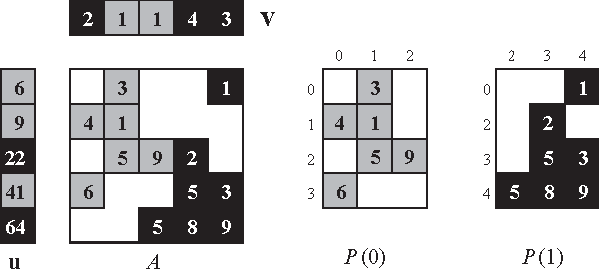
\includegraphics{img/partition}
	\caption{Example of a possible distribution among 2 processors of a 5x5 matrix, and the input and output vectors, as taken from \cite[Fig. 4.3]{BSP}}
		\label{fig:partition}
\end{figure}


After this distribution, each processor has then to compute its local contribution toward the matrix-vector multiplication: to do so, it requires the appropriate vector component, which might have been assigned to another processor during the previous data distribution phase; if this is the case, some communication is required. After the processor has all the required vector components, it starts computing all its local distribution, once this computation step has finished, such local contributions are to their appropriate ``owner'' (according to the distribution of $u$).

These three phases for each processor (whose identity is denoted by the letter $s$) are summarized in Algorithm \ref{alg:matvec}.

\begin{algorithm}[h]
	\begin{algorithmic}
		\Require{$A_s$, the local part of the vector $v$}
		\Ensure{The local part of the vector $u$}
		\State
		\State 	$I_s := \left\{ i | a_{ij} \in A_s \right\}$
		\State 	$J_s := \left\{ j | a_{ij} \in A_s \right\}$
		\State
	\end{algorithmic}
	\begin{enumerate}[(1)]
			\setcounter{enumi}{-1}
		\item 	\begin{algorithmic} \Comment{Fan-out}
				\ForAll{$j \in J_s$}
				\State Get $v_j$ from the processor that owns it. 
				\EndFor
				\State
			\end{algorithmic}
		\item
			\begin{algorithmic} \Comment{Local sparse matrix-vector multiplication}
				\ForAll{$i \in I_s$}
				\State $u_{is} :=0$
				\ForAll{$j$ such that $a_{ij} \in A_s$}
				\State $u_{is} = u_{is} + a_{ij}v_j$
				\EndFor
				\EndFor
				\State
			\end{algorithmic}
		\item
			\begin{algorithmic} \Comment{Fan-in}
				\ForAll{$i \in I_s$}
				\State Send $u_{is}$ to the owner of $u_i$.
				\EndFor
				\State
			\end{algorithmic}
	\end{enumerate}
	\label{alg:matvec}
	\caption{Parallel sparse matrix-vector multiplication.}
\end{algorithm}

In reality there is also a fourth phase, in which each processor sums up all the contributions received in phase (2) for all of its own components of $u$; this is a very small sum with negligible computational cost and for this reason it has been omitted from the algorithm.

Our parallel algorithm, which follows the Bulk Synchronous Parallel model\cite{bsp_paper}, consists of one communication superstep, followed by a computation superstep and finally another communication superstep.

\section{Hypergraph model and current literature}
\section{Medium-grain model}
